
\chapter{Gráficas de Funciones con Discontinuidades}
\chaptermark{Gráficas con Discontinuidades}

\begin{bibunit}[plain]

Para poder generar gráficas de funciones de este tipo, la opción
\emph{discont=true} nos permite indicar a \emph{Maple} que éstas deben eliminarse de la
gráfica. La forma en la que incluimos esta opción es la siguiente:

\begin{verbatim}
plot(funcion(x), x = intervalo, {rango}, discont = true);
\end{verbatim}

Por ejemplo, la siguiente instrucción nos permite desplegar una gráfica de la 
función \emph{tan(x)}:

\begin{verbatim}
plot(tan(x), x = -10 .. 10, -50 .. 50, discont = true);
\end{verbatim}

La gráfica se puede ver en la figura \ref{cap2f1}.

\begin{figure}[h!]
\centering
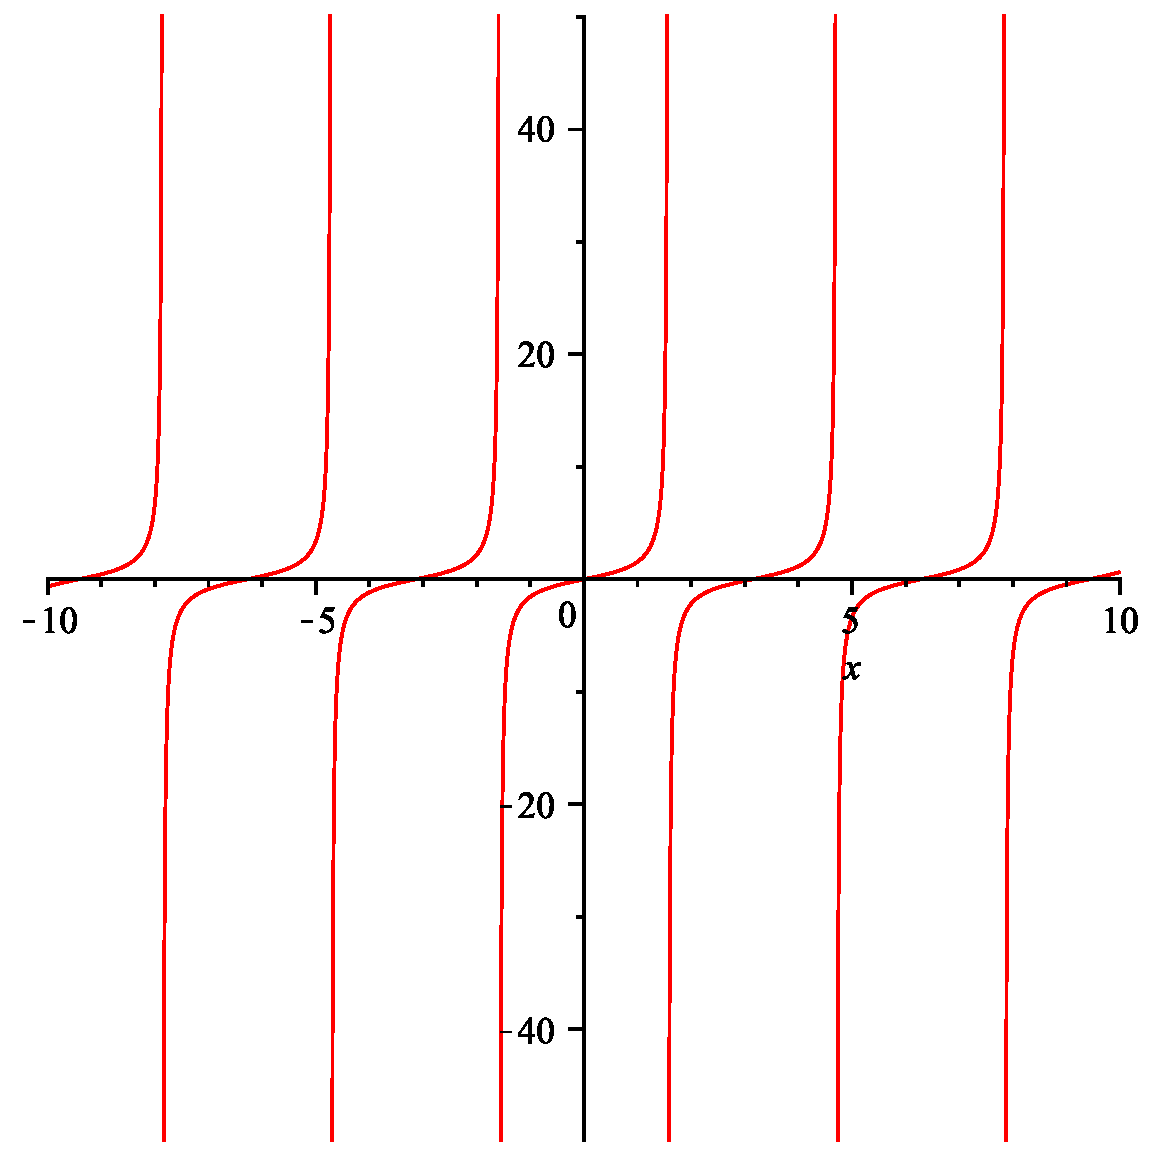
\includegraphics[scale=0.4]{grafica04}
\caption{Gráfica de $tan (x)$}\label{cap2f1}
\end{figure}

Consulte \cite[cap. 2]{spivakCalc} para aprender algo de límites.

\LaTeX{} es un sistema para la composición de documentos \cite[cap. ~2]{Lamport} para aprender algo de \LaTeX{}.

\putbib[mibiblio]

\end{bibunit}

